\justifying

\section*{\textbf{Task 1}:}

 All the variables are initialized by running the provided script "initialization.m”  so that the variables in simulink can refer to the work space for values.

\section*{\textbf{Task 2}:} 
The PMU SCADA blocks are integrated to measure the variation of parameters in this task. The model is then simulated to find the power flow.
\begin{figure}[H]
    \centering
        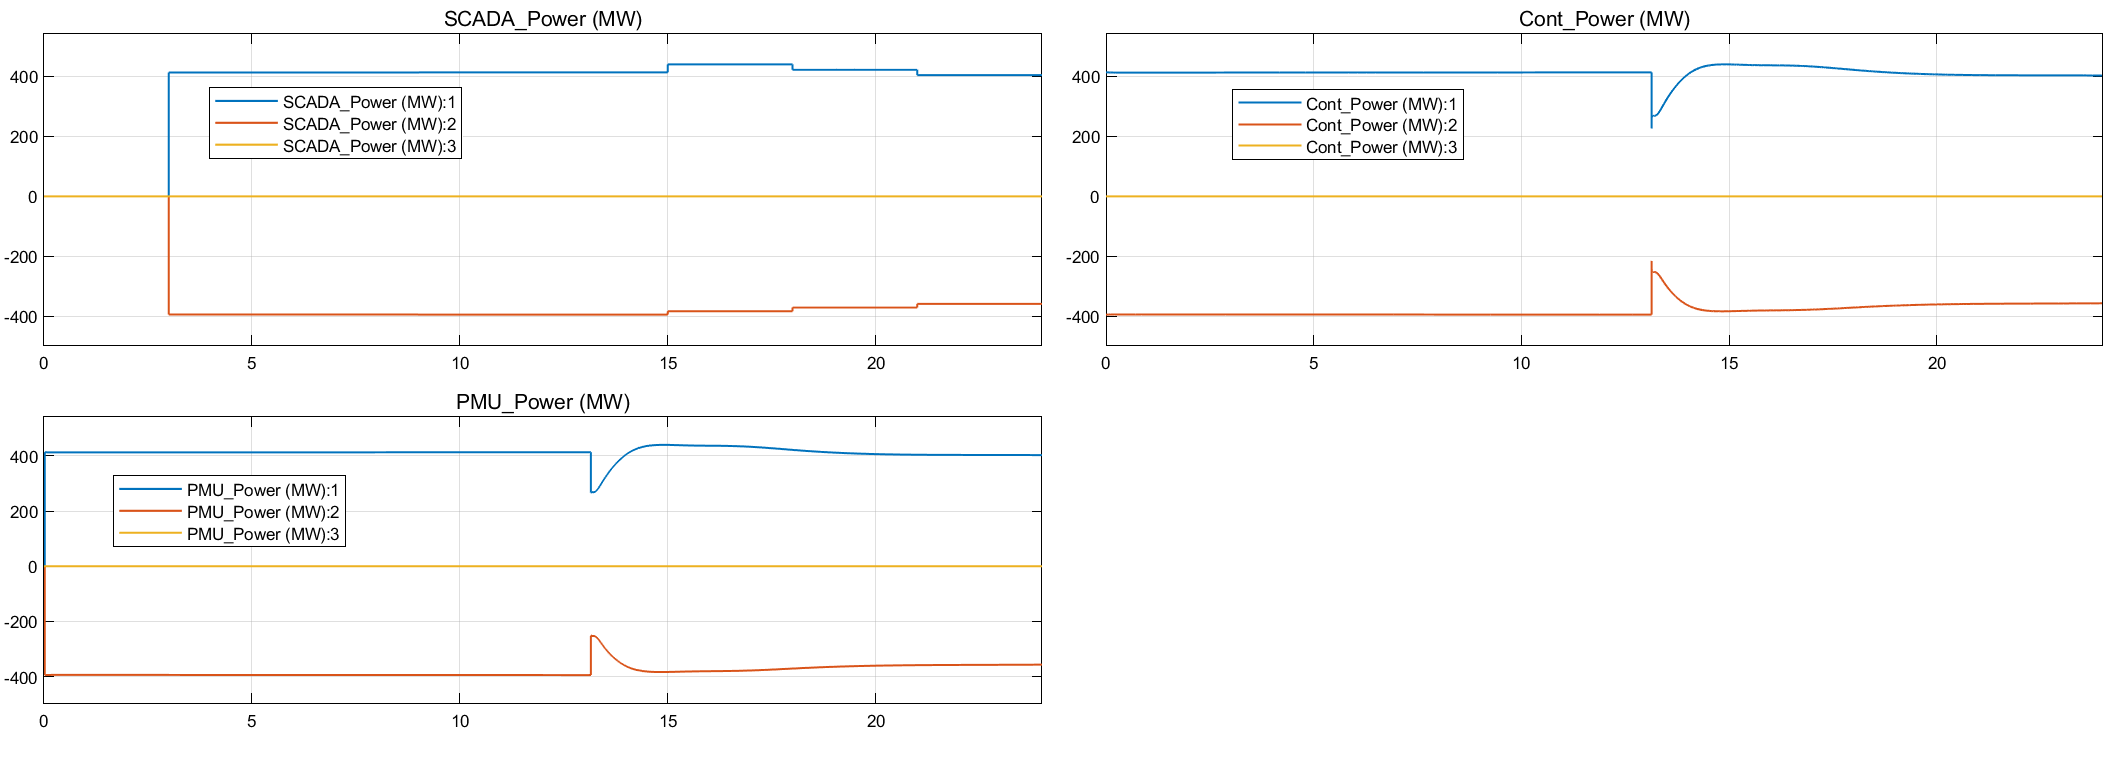
\includegraphics[width=0.8 \linewidth]{images_a4/T2.png}
        \caption{Power flow during normal condition}
        \label{fig:Power flow normal}   
\end{figure}
The power flow is happening from area 1 to area two and this can be seen from \ref{fig:Power flow normal} , the area 1 active shows a positve value of about 410 MW, whereas it is negative in area 2 and the bus voltage to the second bus is hgher than the first.
The power flow variations in SCADA and PMU show some dissimilarities, this can be attributed to the latency of SCADA measurements. PMU measurements provide us more accurate data with regards to system dynamics because of a better resolution of measurement, whereas SCADA cannot capture them.

\section*{\textbf{Task 3}:} In this task a 3 phase  to ground  fault in the middle of the 220 km Line 1  is simulated, and corresponding breakers on both Line 1 ends are enabled such that line 1 is permanently disconnected after the fault (only phase c from left side connected).The power in area 1 reduces due to the occurrence of the fault. Post the fault the system tries to get back to a stable state by balancing the current power flow, the time to do so depends on the magnitude of the transients induced due to the fault.
The PMU is able to capture the intricate system dynamics variation, whereas SCADA is not able to, and hence it proves that if system dynamics has to be analyzed then only PMU measurements can be considered. This can be clearly seen in the \ref{fig:machine_faultl}.

\begin{figure}[H]
    \centering
        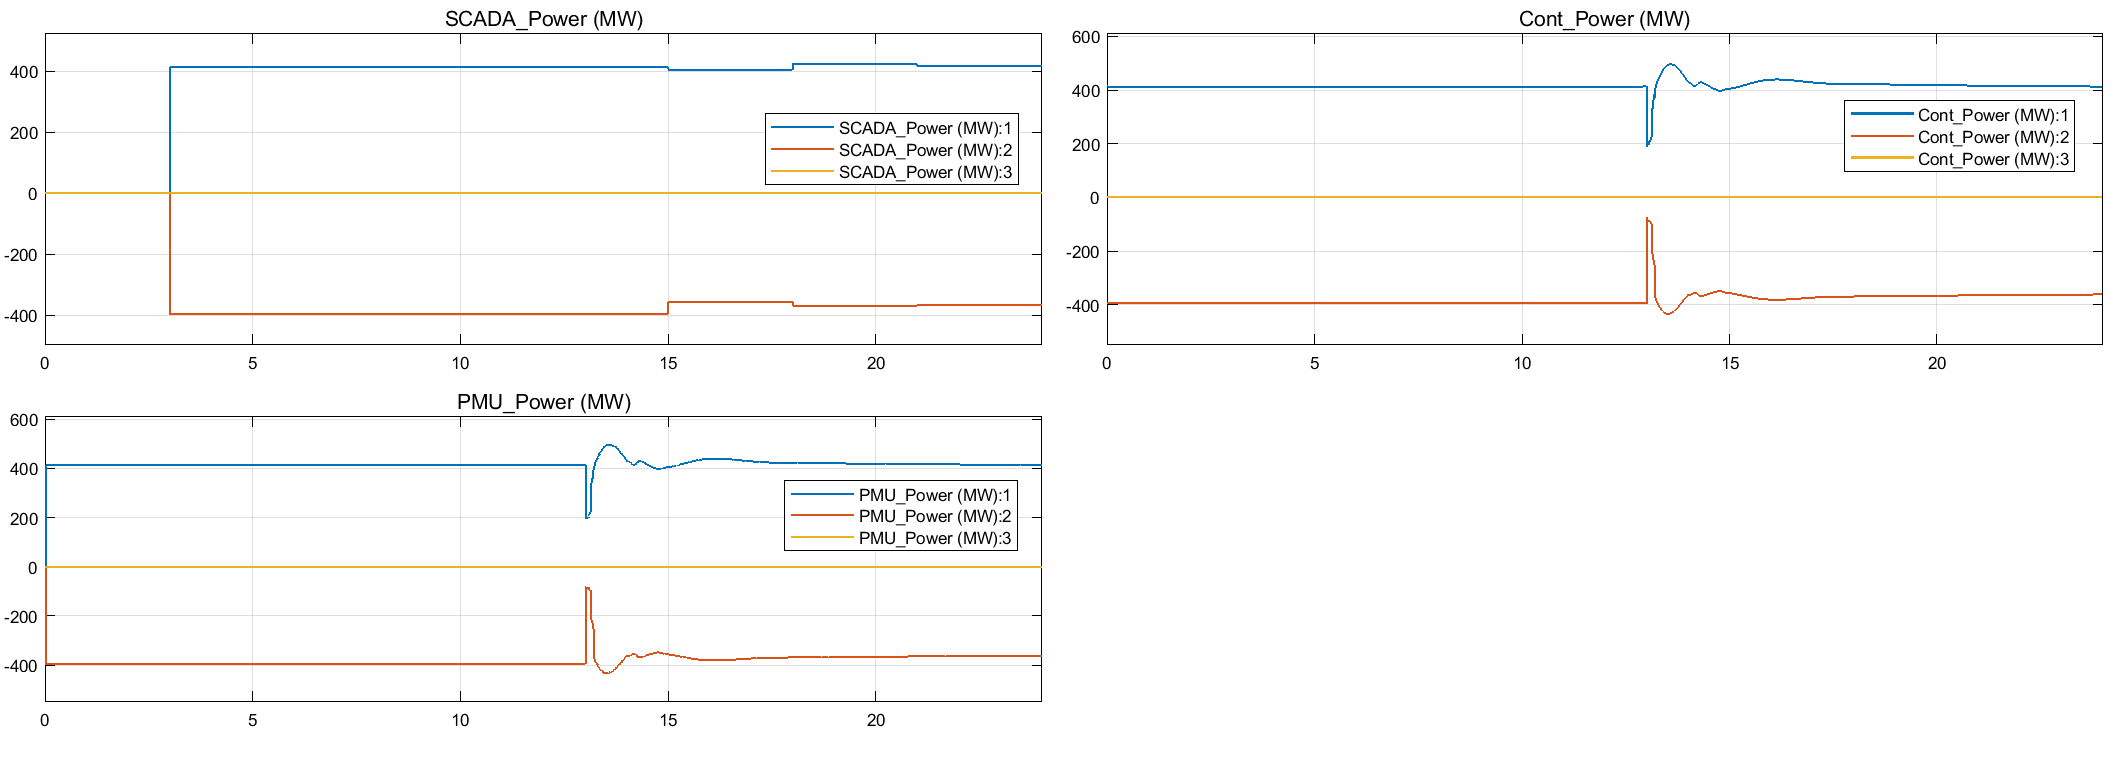
\includegraphics[width=0.8 \linewidth]{images_a4/Q2.png}
        \caption{Power flow during fault}
        \label{fig:Power flow normal}   
\end{figure}
\begin{figure}[H]
    \centering
        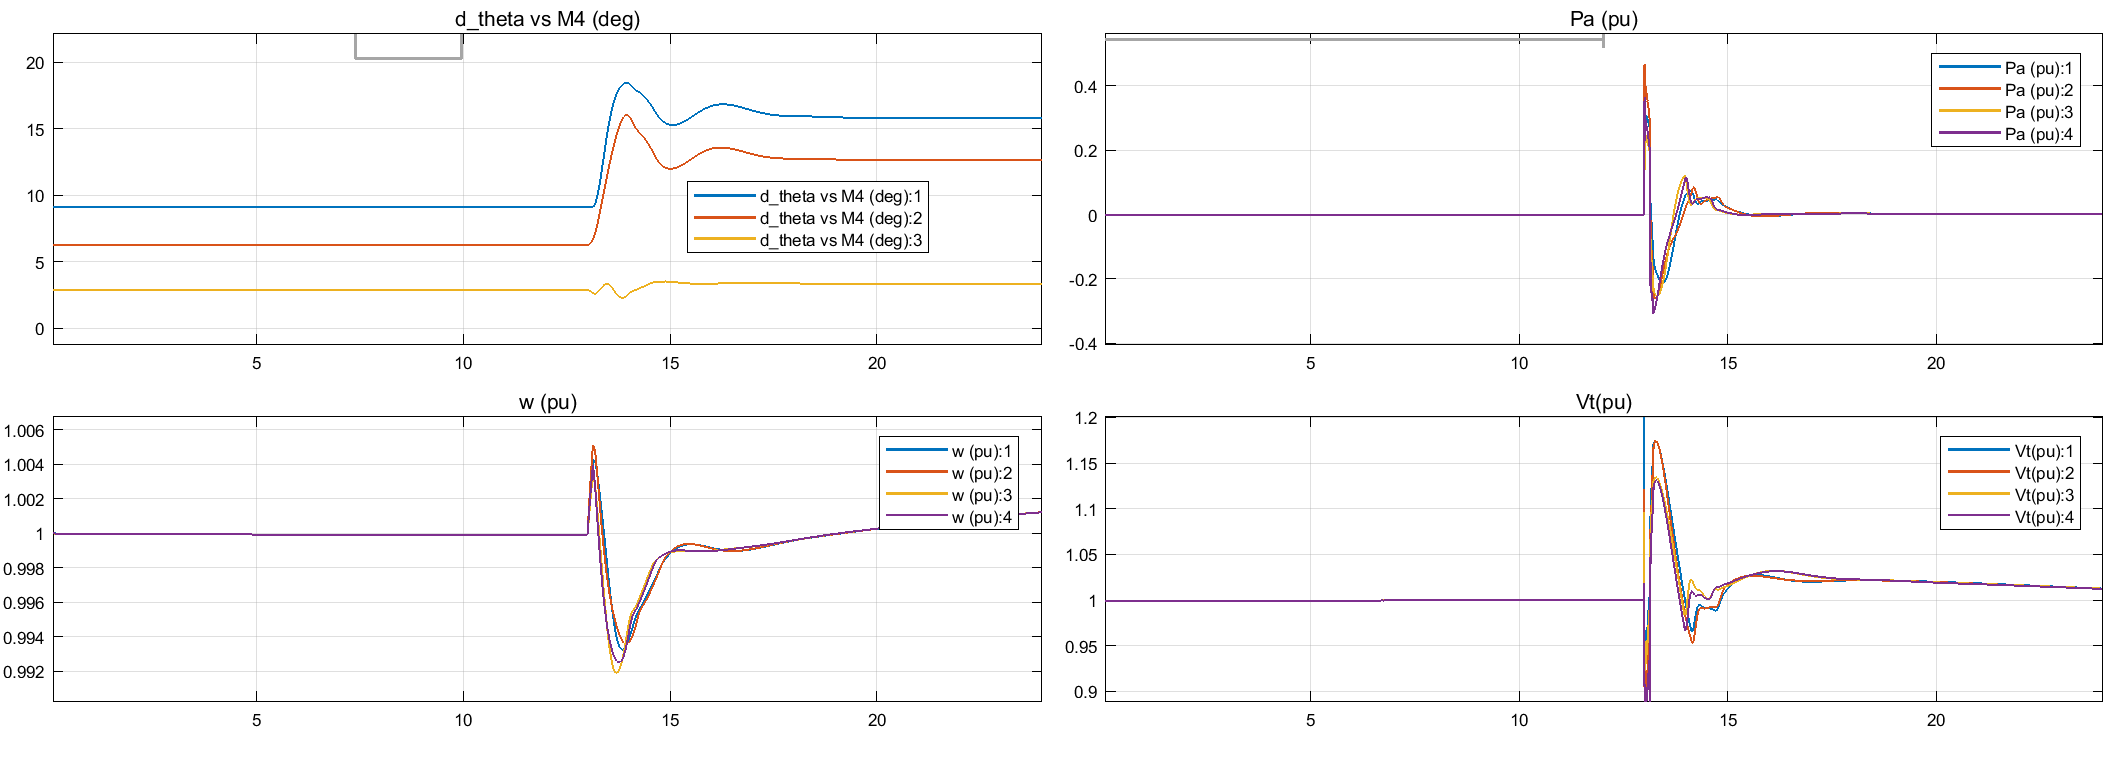
\includegraphics[width=0.8 \linewidth]{images_a4/Q2_m.png}
        \caption{Machine parameters during fault}
        \label{fig:machine_faultl}   
\end{figure}
Post occurrence of the fault the system loses its stability this is evident from \ref{fig:machine_faultl} where the rotor speed and angle are changing, and as we know from swing equation that if there is a change in the rotor angle, there will be an imbalance between Pmech and Pele which leads to transients in the system, it can also cause incoherence in the system.

\section*{\textbf{Task 4}:}
There seems to be a lower system stability with respect to previous cases, and this is because the area 3 has a lot of renewables and this reduces the system inertia and the total reactive power in the system also reduces which affects the voltage stability in the local areas, all the points stated above can be visible from  the figure stated below.

\begin{figure}[H]
    \centering
        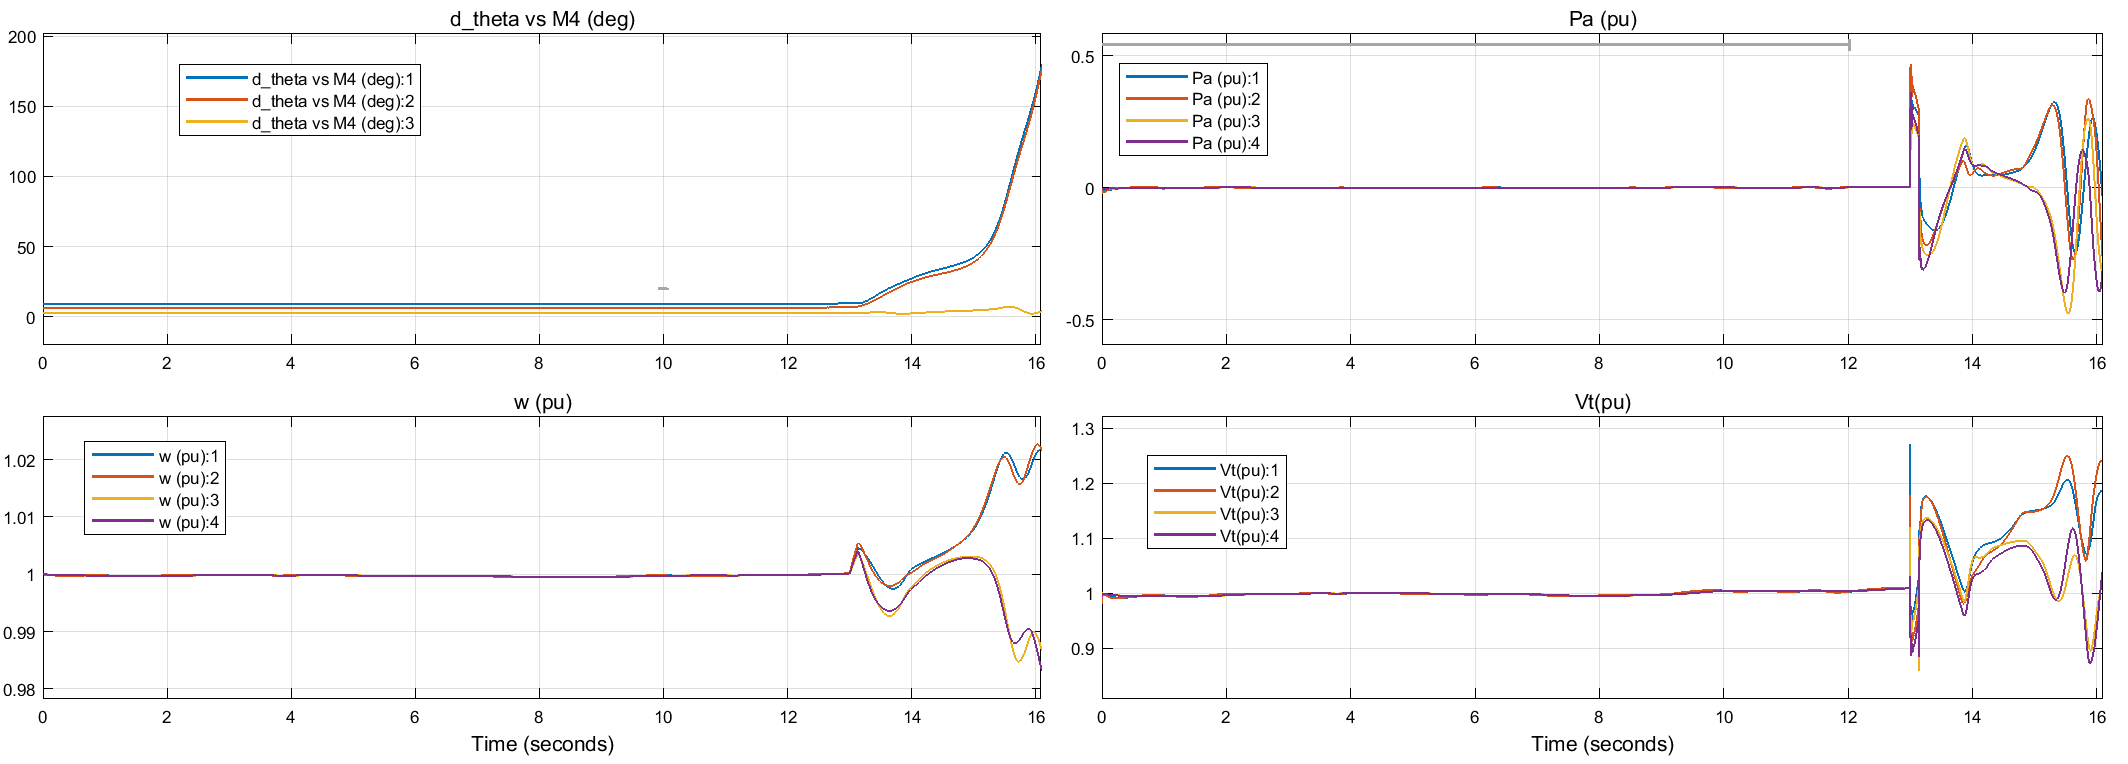
\includegraphics[width=0.8 \linewidth]{images_a4/T4_m.png}
        \caption{Machine parameters during A3 activation}
        \label{fig:machine_t4}   
\end{figure}

\begin{figure}[H]
    \centering
        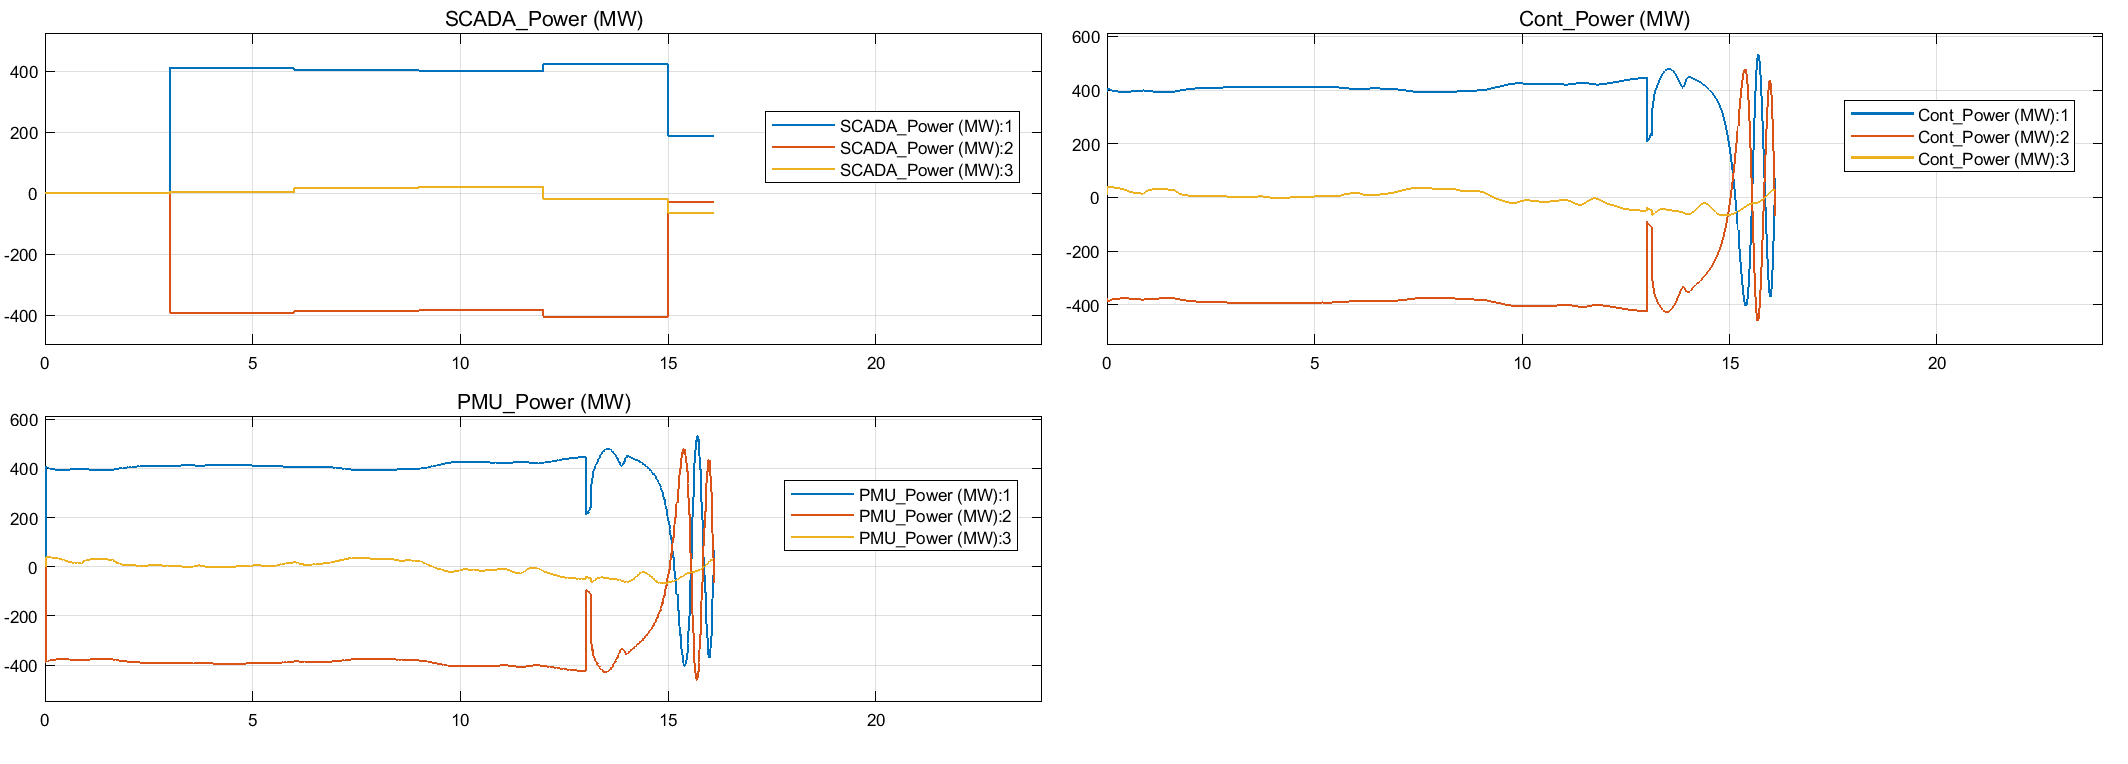
\includegraphics[width=0.8 \linewidth]{images_a4/T4.png}
        \caption{Power flow during A3 activation}
        \label{fig:machine_t4}   
\end{figure}
As the demand varies, the active power is also varied, this causes a change in frequency of the rotors and also affects the rotor angles, post stabilization of the demand the parameters can be seen to settle down.
When the fault occurs huge variations can be observed in area 1 and 2 because the fault is occuring between them.There is an uncontrolled rise in the frequency of the machines and hence to prevent the physical failure of the system, the Generator circuit breaks of the generator disconnects it from the system to prevent the failure of the machine.The system control and protection devices is reason why the simulation fails after 17 seconds, since there are no more generators in the system to solve the power flow for.
\section*{\textbf{Task 5}:}
Initially the fault which occurs at 13 s is cleared at around 13.3 seconds. If the battery controller uses the SCADA measurements as a reference for control it can be detrimental to the entire system,Since the battery balances per second energy balance it is important for the battery controller to have data with high resolution and hence we prefer using PMU measurements over SCADA for the battery control, and since there is dearth of inertia in the system due to the excess of renewable sources it is important for the battery to provide a fast response.
To overcome the problems stated above and increase the stability of the system PMU measurements must be used as reference to the battery controller.

\begin{figure}[H]
    \centering
        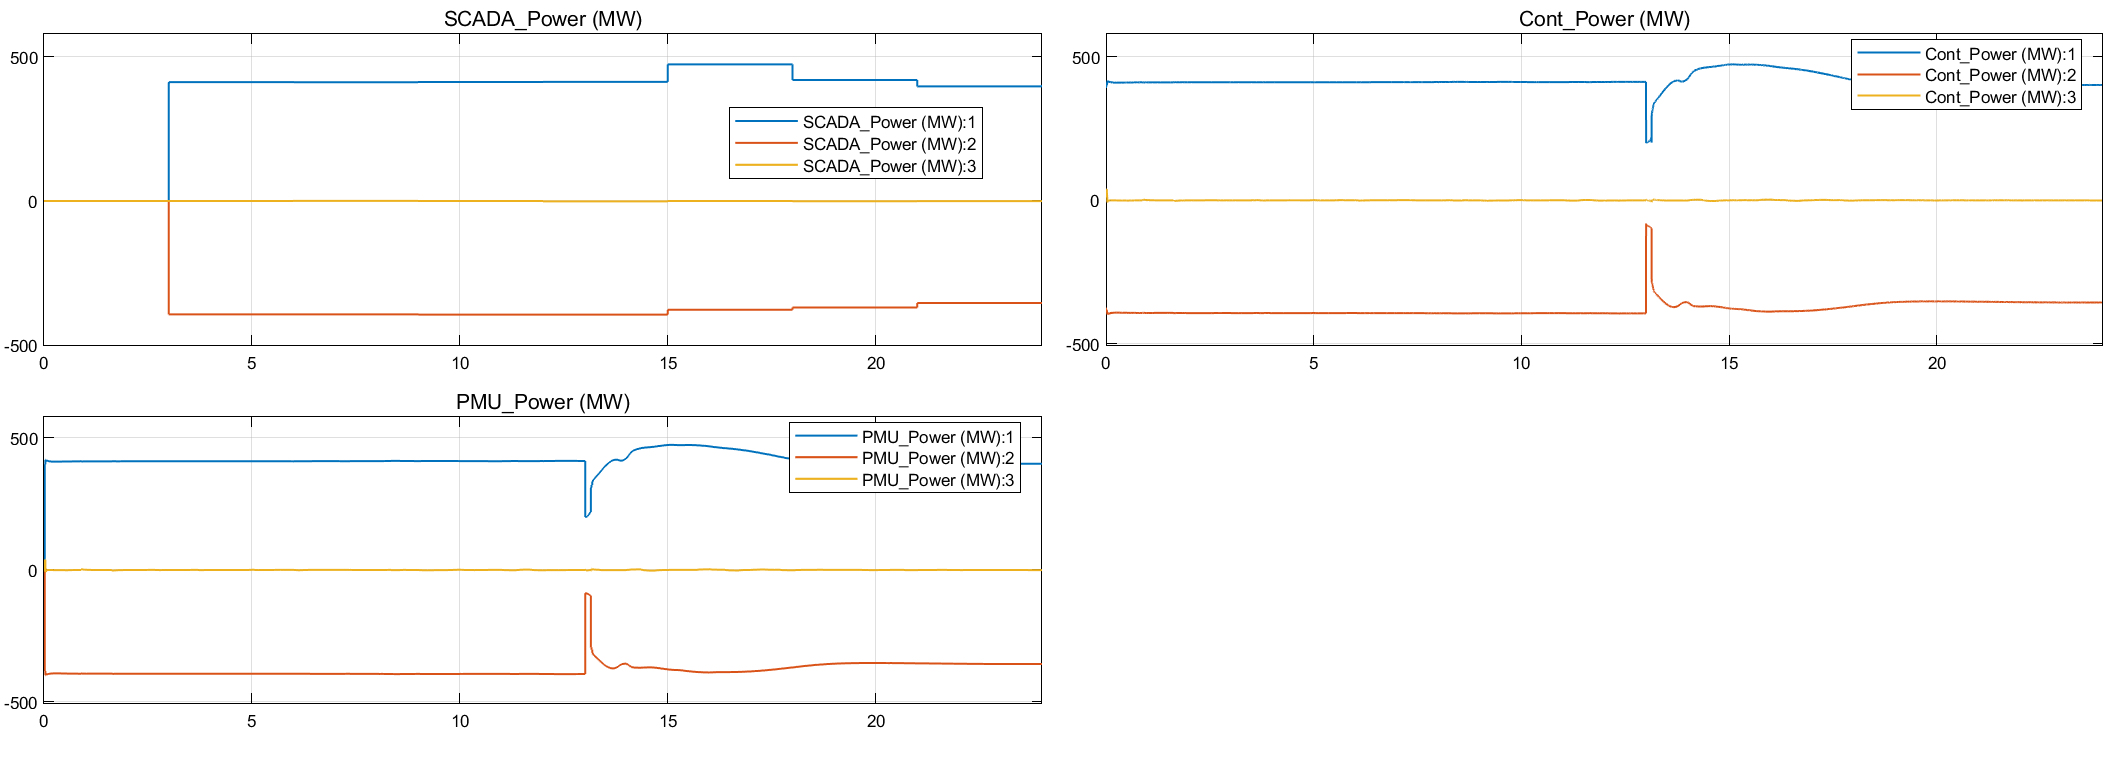
\includegraphics[width=0.8 \linewidth]{images_a4/T5_PMU.png}
        \caption{PMU measurements}
        \label{fig:PMU}   
\end{figure}
\begin{figure}[H]
    \centering
        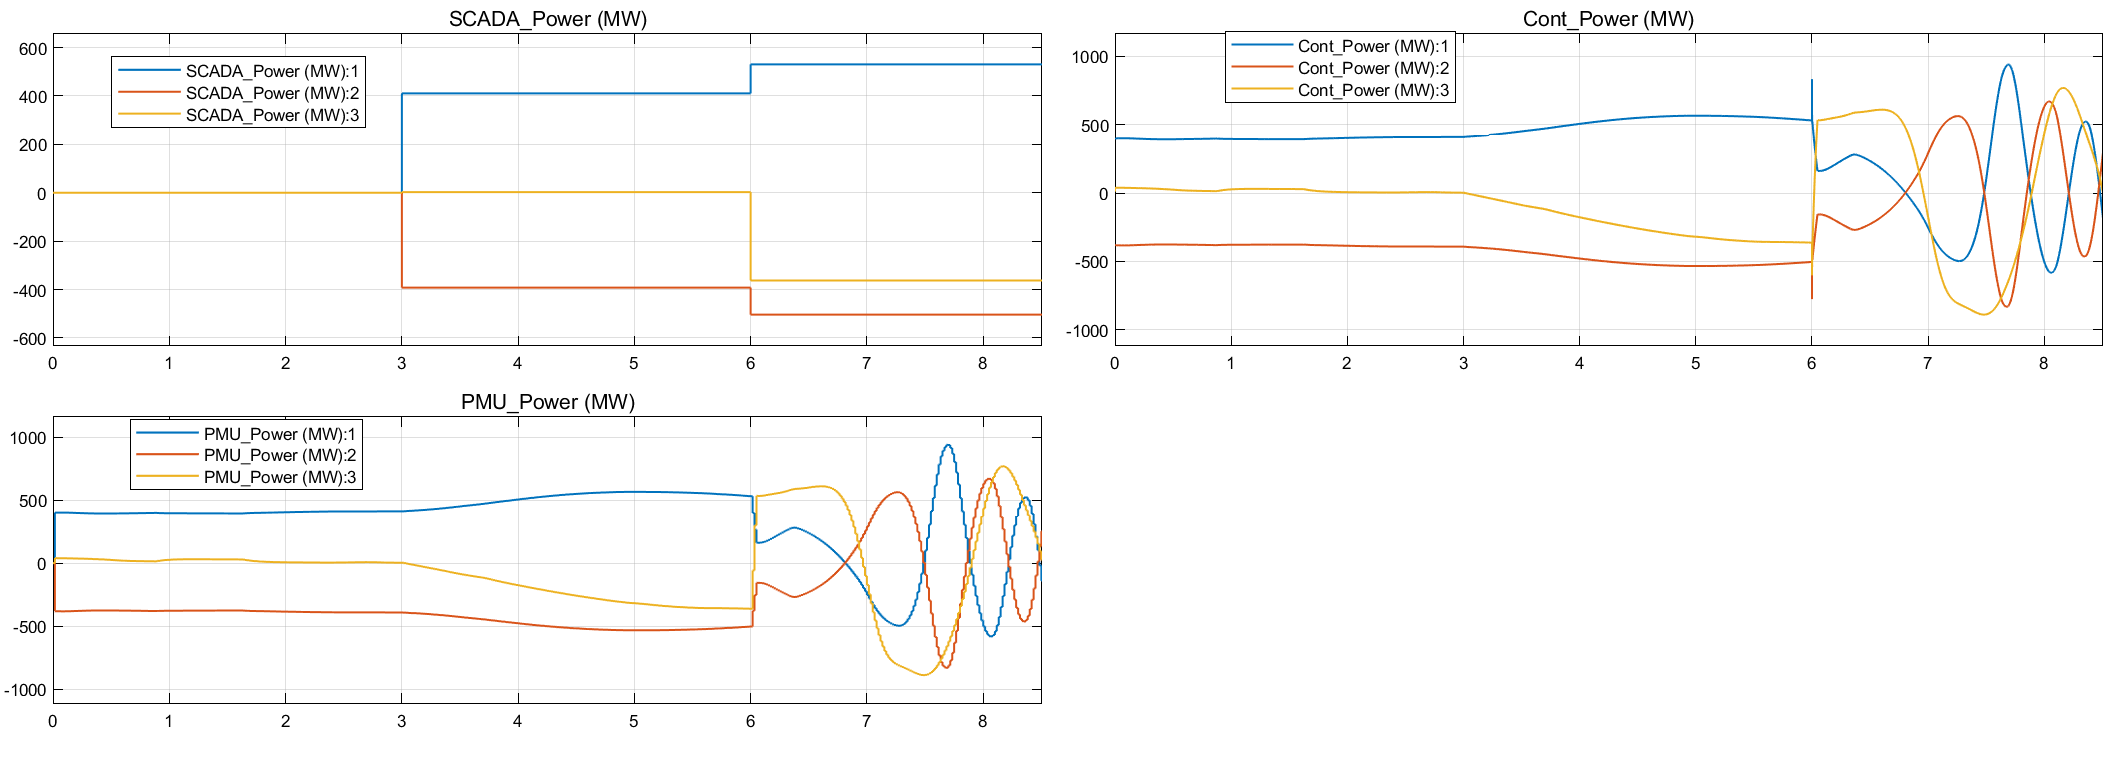
\includegraphics[width=0.8 \linewidth]{images_a4/T5_SCADA.png}
        \caption{SCADA  measurements}
        \label{fig:SCADA}   
\end{figure}

\section*{\textbf{Task 6}:}

It was observed that the model fails to simulate when the battery control is done through SCADA as opposed to PMU. The reason for this, is the amount of time taken by both of these to retrieve the data. For PMU it was 60 fps whereas for SCADA it was 3 seconds. 3 seconds being a significantly long duration can lead to loss of critical data.
All the sources in area 3 being renewable, lead to a unsteady generation of power. This overall results in fluctuating output from area 3. PMU being more fast, is able to function and provide the battery controller with the necessary information for a better operation. Whereas the SCADA being inherently slow, fails to gather information and results in system collapse. The presence of fault alongside a large fluctuation of power leads to an increase in the rotor speed which causes the system to fail.
The continuous type of signal required for the controller to work properly are not available in reality. In order to achieve a similar behaviour one try and minimize the time interval required to receive the data. But making that delay to be zero is not possible in reality.
More cost effective ways to increase the PMU's ability to gather the data can be implemented.

To overcome the issue in Task 4 a better control strategy to deal with the integration of renewable sources can be implemented.It can be ensured that there is a better frequency control available, which can deal with the variable nature of such sources. 

